\documentclass[fleqn,final]{jaes}

% Metadata Information
\jyear{2026}
\jmonth{November}
%\jvol{72}
%\jnum{11}

\usepackage{amsmath}\setlength{\mathindent}{19pt}
\usepackage{bm}
\usepackage{booktabs}
\usepackage[final]{graphicx}
\graphicspath{{./}{figures/}}
\usepackage{url}
\usepackage{hyperref}
\hypersetup{
  pdfauthor={Boobalan Arjunan},
  pdftitle={Real-Time Circuit-Based Audio Synthesis Using Modified Nodal Analysis: Feasibility, Signal Continuity, and Storage Trade-Offs},
  pdfkeywords={Modified Nodal Analysis, Virtual Analog Synthesis, AudioWorklet, Newton-Raphson, Parameter Continuity, Procedural Audio},
  hidelinks
}
\usepackage[capitalize]{cleveref}

% Safeguard against draft-mode cached line numbers in output.aux
\makeatletter
\providecommand{\@LN@col}[1]{}
\providecommand{\@LN}[2]{}

\makeatother


% Safeguard against template-level author macros or trailing hooks
\makeatletter
\providecommand{\@LN@col}[1]{}
\providecommand{\@LN}[2]{}
\def\theauthors{}
\def\THEAUTHORS{}
\let\theauthors\relax
\let\THEAUTHORS\relax
\makeatother

\begin{document}

% Title portion (Max 125 characters, no 'new' or 'novel')
\title{Real-Time Circuit-Based Audio Synthesis Using Modified Nodal Analysis: Feasibility, Signal Continuity, and Storage Trade-Offs}

% Page heads (Authors) (Short title)
\markboth{ARJUNAN}{REAL-TIME CIRCUIT-BASED AUDIO SYNTHESIS USING MNA}

% Author Information
\authorgroup{
  \author{BOOBALAN ARJUNAN\thanks{To whom correspondence should be addressed, email: boobalan\_arjunan@composermind.com.}}
  \email{(boobalan\_arjunan@composermind.com)}
  \affil{
    ComposerMind Labs, Chennai, India
  }
}

\maketitle

\begin{abstract}
\noindent Interactive spatial audio engines must meet fixed audio-processing deadlines, maintain minimal memory footprints, and deliver responsive modulation under continuous parameter sweeps. Conventional multi-sample playback demands substantial storage for multi-zone parameter coverage and can introduce phase cancellation during crossfading. This paper evaluates discrete-time Modified Nodal Analysis (MNA) with iterative Newton--Raphson non-linear solving in Web Audio \texttt{AudioWorkletProcessor} architectures. High-resolution profiling on an ARM64 Apple M1 Max host demonstrated that steady-state 4-voice MNA consumes an average of 10.31\% to 22.98\% (612.7~$\mu$s) of the 2,666.67~$\mu$s block deadline across an 18,000-block factorial benchmark, with zero deadline violations observed during testing (peak transient duration: 1,704.7~$\mu$s, 36.07\% headroom). In a dedicated 20-trial evaluation, preallocated cold-start blocks completed within 873.4~$\mu$s. Under a 60~Hz parameter sweep across 20 trials, in-place reactive state preservation produced significantly fewer first-derivative outlier spikes than a matched 3-zone sample-crossfade baseline ($t = -6.64, p = 2.37 \times 10^{-6}$). The verified 61-preset netlist library occupies 81,130 bytes of persistent source assets, representing a $12,992\times$ to $76,223\times$ storage reduction compared to modeled uncompressed PCM sample banks (1.05 to 6.18~GB) and $860\times$ to $1,170\times$ versus lossy compressed audio (70 to 95~MB), balanced against an approximately $8\times$ higher computational cost during active modulation ($152.7\,\mu\text{s}$ vs. $19.0\,\mu\text{s}$ in 1-voice testing; polyphonic ratios in steady-state range from $4.9\times$ to $11.1\times$).
\end{abstract}

\begin{keywords}
Modified Nodal Analysis, Virtual Analog Synthesis, Physical Modeling, AudioWorklet, Newton--Raphson, Parameter Continuity, Procedural Audio, Audio for Extended Reality
\end{keywords}

\noindent\textbf{JAES Thematic Section:} 14.~Interactive audio

\section{INTRODUCTION}

Interactive spatial computing, gaming, and Extended Reality (XR) require audio engines that respond dynamically to continuous user input, including 60~Hz or 120~Hz hand-tracking gestures, 6-DOF head motion, and controller manipulation. In these applications, synthesis engines must operate within deterministic real-time audio thread deadlines---conventionally 128 samples per block at 48~kHz ($2.67\text{ ms}$)---while sharing memory and processing resources with concurrent tracking, computer vision, and rendering tasks.

For interactive virtual instrument and sound-asset playback in games and simulation, the predominant architecture remains \textbf{multi-sample playback}. Sample playback is computationally lightweight, requiring only table lookups, fractional delay interpolation, and gain scaling. However, scaling sample playback to support multi-dimensional, continuous parametric interaction (such as sweeping a circuit's drive, resistance, or resonance) presents two primary challenges:
\begin{enumerate}
\item \textit{Asset Storage and Memory Pressure:} Capturing non-linear parametric variations requires dense grids of multi-samples across pitch, velocity, and control axes. On resource-constrained embedded systems, storing and streaming multi-gigabyte sample libraries strains disk storage and unified memory architectures.
\item \textit{Crossfading Artifacts:} When transitioning between discrete parameter zones under continuous control, sample engines typically employ equal-power crossfading. Because independently recorded audio samples have uncorrelated phase trajectories, crossfading can cause phase cancellation, comb filtering, and timbral stepping unless extensive control-rate low-pass smoothing is applied \cite{serafin2016virtual, turchet2021smart}.
\end{enumerate}

\textbf{Procedural physical modeling}, and specifically discrete-time circuit simulation via Modified Nodal Analysis (MNA), synthesizes waveforms directly from mathematical descriptions of electrical circuits. By updating component conductances in-place while preserving the internal energy states of reactive components (capacitors and inductors), physical models can inherently generate smooth timbral transitions without requiring pre-recorded audio assets. Historically, non-linear MNA solvers---which require iterative matrix solutions at every audio sample---have been considered computationally demanding for real-time consumer deployment, particularly within web-based or mobile runtime environments.

This paper investigates the computational and storage trade-offs of real-time circuit-based synthesis, focusing on the following central research question:
\begin{quote}
\textit{Can state-preserving, circuit-based procedural synthesis support rapid interactive parameter changes while offering a practical compute--storage trade-off against multi-sample playback?}
\end{quote}

We evaluate the discrete-time MNA engine implemented in NodalSynth Pro, designed for execution in the Web Audio \texttt{AudioWorkletProcessor} environment. Host measurements were conducted on an Apple M1 Max host using headless V8 microsecond timing, accompanied by browser-level execution verification in Chromium. We measure block-by-block processing execution times, quantify parameter continuity under a 60~Hz control sweep against a matched multi-zone sample-crossfade baseline, audit the exact binary netlist storage, and project modeled storage requirements for equivalent multi-sample representations. All test scripts, measurement datasets, and the interactive HTML benchmark suite are publicly available under the open-source MIT license at: \url{https://github.com/BoobalanArjunan/Real-Time-Circuit-Based-Audio-Synthesis}.

\section{RELATED WORK}

\subsection{Virtual Analog Circuit Modeling and MNA}
Virtual analog (VA) modeling aims to digitize acoustic and electronic instruments by discretizing physical circuit equations. Foundational techniques encompass Wave Digital Filters (WDF), state-space formulations, and Modified Nodal Analysis (MNA). While WDFs \cite{fettweis1986wave, smith2010physical} decouple reciprocal circuit elements through wave variables, they can become complex when handling arbitrary multi-port non-linear topologies. State-space approaches \cite{bilbao2009numerical, valimaki2006discrete} provide compact mathematical representations but require explicit derivation of state-variable differential equations.

Modified Nodal Analysis, originally formulated by Ho, Ruehli, and Brennan \cite{ho1975modified}, provides a systematic method for generating circuit equations directly from schematic netlists using Kirchhoff's Current Law (KCL) and branch equations. Yeh, Abel, and Smith \cite{yeh2007automated, yeh2009automated} demonstrated the viability of automated MNA solvers for non-linear audio circuits, including guitar distortion stages, showing that Newton--Raphson iteration can solve transcendental diode equations in discrete time. Further advances by Holters and Z\"olzer \cite{holters2011physical, holters2015combined} explored parameterized multi-port models and iterative solvers for vacuum-tube amplifiers. While these prior studies established the theoretical foundation of circuit simulation for audio effects, their implementations were predominantly designed for offline simulation or compiled C/C++ audio plugins running on desktop workstation CPUs.

\subsection{Web Audio and AudioWorklet Architectures}
The evolution of the W3C Web Audio API \cite{w3c2021webaudio} from early script processor nodes to the \texttt{AudioWorklet} architecture \cite{choi2018audioworklet} enabled custom, low-latency DSP execution directly on a dedicated real-time audio rendering thread. Choi \cite{choi2018highperformance} and Adenot et al. \cite{adenot2015webaudio} demonstrated that modern Just-In-Time (JIT) JavaScript engines (such as V8) can achieve predictable real-time DSP performance in browser environments, provided memory allocations inside the audio callback are avoided to prevent garbage collection (GC) pauses. Recent work has explored running physical models and compiled WebAssembly (Wasm) modules in \texttt{AudioWorklet} \cite{buffa2019webaudio}, but systematic evaluations of polyphonic non-linear MNA solvers under strict audio block deadlines remain limited in the literature.

\subsection{Procedural Audio and Extended Reality (XR) Constraints}
Procedural audio generates sound dynamically through computational models rather than replaying static recordings \cite{farnell2010designing}. In virtual reality (VR) and extended reality (XR), procedural sound offers advantages for interactive objects, physical collisions, and continuous spatial interaction \cite{serafin2016virtual, turchet2021smart}. Serafin et al. \cite{serafin2016virtual} emphasized that VR musical instruments and interactive sound objects demand continuous physical responsiveness without discrete velocity or layer stepping. In mobile and standalone XR platforms, audio rendering must share strict CPU, thermal, and memory budgets with head tracking, spatial mapping, and graphics rendering \cite{poletti2016spatial, armstrong2020audio}. While spatialization pipelines (e.g., binaural HRTF convolution and room acoustics simulation) have been widely investigated \cite{poletti2016spatial, ziegelwanger2015numerical}, the compute--storage trade-offs of the underlying source sound generators under real-time interactive constraints warrant empirical evaluation.

\section{MATHEMATICAL FORMULATION OF THE MNA SOLVER}

\subsection{Modified Nodal Analysis (MNA) Formulation}
Following the standard MNA formulation \cite{ho1975modified, yeh2007automated}, an electrical network containing $N$ ungrounded nodes and $K$ independent voltage sources is described by:
\begin{equation}
\mathbf{A} \mathbf{x}(t) = \mathbf{z}(t)
\end{equation}
where $\mathbf{x}(t) = \begin{bmatrix} v_1 & \dots & v_N & i_{E1} & \dots & i_{EK} \end{bmatrix}^T$ is the vector of unknown node voltages and voltage-source branch currents. The system matrix $\mathbf{A} \in \mathbb{R}^{M \times M}$ ($M = N + K$) is partitioned into:
\begin{equation}
\begin{bmatrix} \mathbf{G} & \mathbf{B} \\ \mathbf{C} & \mathbf{D} \end{bmatrix} \begin{bmatrix} \mathbf{v}(t) \\ \mathbf{i}_E(t) \end{bmatrix} = \begin{bmatrix} \mathbf{j}(t) \\ \mathbf{e}(t) \end{bmatrix}
\end{equation}
where $\mathbf{G}$ represents static node conductances, $\mathbf{B}$ and $\mathbf{C}$ describe voltage-source incidence ($\mathbf{C} = \mathbf{B}^T$ for reciprocal networks), $\mathbf{D}$ is zero for ideal independent sources, and the right-hand vector $\mathbf{z}(t) = \begin{bmatrix} \mathbf{j}(t) & \mathbf{e}(t) \end{bmatrix}^T$ incorporates source excitations and reactive companion currents.

\subsection{Discrete-Time Companion Models}
Linear reactive elements (capacitors and inductors) are discretized at sample period $T = 1 / f_s$ using the bilinear transform (Trapezoidal integration rule).

\subsubsection{Capacitor Companion Model}
The continuous-time constitutive relation $i_C(t) = C \frac{dv}{dt}$ discretized via the trapezoidal rule yields:
\begin{equation}
v[n] - v[n-1] = \frac{T}{2C} \left( i_C[n] + i_C[n-1] \right)
\end{equation}
Rearranging into the Norton equivalent companion form implemented in the engine:
\begin{equation}
i_C[n] = G_{\text{eq}, C} \left( v[n] - v[n-1] \right) - i_C[n-1]
\end{equation}
where the equivalent conductance is:
\begin{equation}
G_{\text{eq}, C} = \frac{2C}{T}
\end{equation}
In the solver's state layout, the voltage difference $v[n-1]$ is tracked in state vector $\mathbf{S}_1$ and previous branch current $i_C[n-1]$ in state vector $\mathbf{S}_2$. During the right-hand side assembly (\texttt{push}), the Norton equivalent history current injected into the system is:
\begin{equation}
I_{\text{eq}, C}[n-1] = G_{\text{eq}, C} \, v[n-1] + i_C[n-1]
\end{equation}
Upon solver convergence (\texttt{commit}), the states are updated:
\begin{align}
i_C[n] &= G_{\text{eq}, C} \left( v[n] - S_1[n-1] \right) - S_2[n-1] \\
S_1[n] &= v[n], \quad S_2[n] = i_C[n]
\end{align}

\subsubsection{Inductor Companion Model}
For an inductor with constitutive relation $v_L(t) = L \frac{di}{dt}$, trapezoidal integration yields:
\begin{equation}
i_L[n] = i_L[n-1] + G_{\text{eq}, L} \left( v[n] + v[n-1] \right)
\end{equation}
where:
\begin{equation}
G_{\text{eq}, L} = \frac{T}{2L}
\end{equation}
The history current injected into the right-hand side vector is:
\begin{equation}
I_{\text{eq}, L}[n-1] = - \left( i_L[n-1] + G_{\text{eq}, L} \, v[n-1] \right)
\end{equation}
Upon convergence, the inductor states are updated:
\begin{align}
i_L[n] &= S_2[n-1] + G_{\text{eq}, L} \left( v[n] + S_1[n-1] \right) \\
S_1[n] &= v[n], \quad S_2[n] = i_L[n]
\end{align}

\subsubsection{Reactive State Preservation}
Unlike sample engines, where voice parameter sweeps require re-triggering or crossfading independent audio buffers, the MNA solver updates conductances in $\mathbf{A}$ while preserving history vectors:
\begin{equation}
\mathbf{S}_C[n] = v_C[n], \quad \mathbf{S}_L[n] = i_L[n]
\end{equation}
Because the stored energy in physical reactive components ($\frac{1}{2}Cv^2$ and $\frac{1}{2}Li^2$) varies continuously as conductance parameters change, the output waveform maintains natural acoustic continuity without phase discontinuities.

\subsection{Non-linear Diode Modeling via Newton--Raphson}
Solid-state diodes are modeled using the Shockley diode equation:
\begin{equation}
i_D(v_D) = I_s \left( \exp\left(\frac{v_D}{\eta V_T}\right) - 1 \right)
\end{equation}
where $I_s$ is reverse saturation current, $\eta$ is the ideality factor, and $V_T$ is the thermal voltage defined as:
\begin{equation}
V_T = \frac{k_B T_K}{q} \approx 25.85\text{ mV}
\end{equation}
where $k_B = 1.380649 \times 10^{-23}\text{ J/K}$ is Boltzmann's constant, $T_K = 300\text{ K}$ is the operating temperature ($V_T \approx 25.26\text{ mV}$ at standard room temperature $293.15\text{ K}$), and $q = 1.60217663 \times 10^{-19}\text{ C}$ is elementary charge. At each discrete time step, the non-linear equation system $\mathbf{F}(\mathbf{x}) = \mathbf{0}$ is solved iteratively via Newton--Raphson:
\begin{align}
\mathbf{J}_{\mathbf{F}}(\mathbf{x}^{(k)}) \, \Delta \mathbf{x}^{(k)} &= - \mathbf{F}(\mathbf{x}^{(k)}) \\
\mathbf{x}^{(k+1)} &= \mathbf{x}^{(k)} + \alpha^{(k)} \Delta \mathbf{x}^{(k)}
\end{align}
The Jacobian dynamic conductance $g_d^{(k)}$ is evaluated at each iteration:
\begin{equation}
g_d^{(k)} = \frac{di_D}{dv_D}\Bigg|_{v_D^{(k)}} = \frac{I_s}{\eta V_T} \exp\left(\frac{v_D^{(k)}}{\eta V_T}\right)
\end{equation}
Iterations proceed until the maximum junction voltage update across non-linear diode ports satisfies $\|\Delta \mathbf{v}_D^{(k)}\|_\infty < \epsilon_{\text{tol}}$ with $\epsilon_{\text{tol}} = 10^{-6}\text{ V}$, or until reaching the iteration cap $k_{\max} = 24$. Dynamic logarithmic damping is applied when forward diode voltages exceed $0.5\text{ V}$, alongside an absolute voltage update clamp of $\pm 20\text{ V}$. Across all $4.608 \times 10^6$ internal oversampled non-linear solves ($18,000\text{ blocks} \times 128\text{ samples} \times 2\times\text{ oversampling}$), $99.88\%$ of individual sample solves converged within $\le 6$ iterations. The 24-iteration cap was reached in only $0.017\%$ of sample solves (affecting $< 0.02\%$ of audio blocks during steep slewing). When the cap is reached, the solver retains the latest bounded estimate $\mathbf{v}_D^{(24)}$ to prevent audio thread overruns while preserving bounded state continuity.

\subsection{Oversampling and Anti-Aliasing Filtering}
To attenuate non-linear aliasing harmonics, the MNA solver executes with internal $2\times$ oversampling ($f_{\text{internal}} = 96\text{ kHz}$ for a $48\text{ kHz}$ audio output). Each audio step solves two internal sub-samples, which are filtered and downsampled using a 23-tap (22nd-order) Blackman-windowed half-band polyphase FIR decimation filter:
\begin{equation}
H(z) = \sum_{k=0}^{22} h[k] \, z^{-k}
\end{equation}
The filter is a linear-phase Type-I half-band FIR filter centered at $k=11$ ($h[11] = 0.5$). The impulse response satisfies the half-band zero condition $h[11 + 2m] = 0$ for $1 \le |m| \le 5$. The non-zero odd-offset coefficients ($m \in \{0, 1, 2, 3, 4, 5\}$) are evaluated from windowed sinc prototypes:
\begin{equation}
h[11 \pm (2m+1)] = \frac{(-1)^m}{\pi (2m+1)} \cdot w[m]
\end{equation}
where $w[m]$ is the 12-point symmetric Blackman window:
\begin{equation}
\begin{aligned}
w[m] &= 0.42 + 0.5 \cos\left(\frac{\pi(2m+1)}{12}\right) \\
&\quad + 0.08 \cos\left(\frac{2\pi(2m+1)}{12}\right)
\end{aligned}
\end{equation}
normalized such that $\sum_{k=0}^{22} h[k] = 1$. This half-band structure identically eliminates half of the multiplication operations during polyphase decimation.

\begin{figure}[t]
\centering
\IfFileExists{figure1_pipeline.pdf}{%
  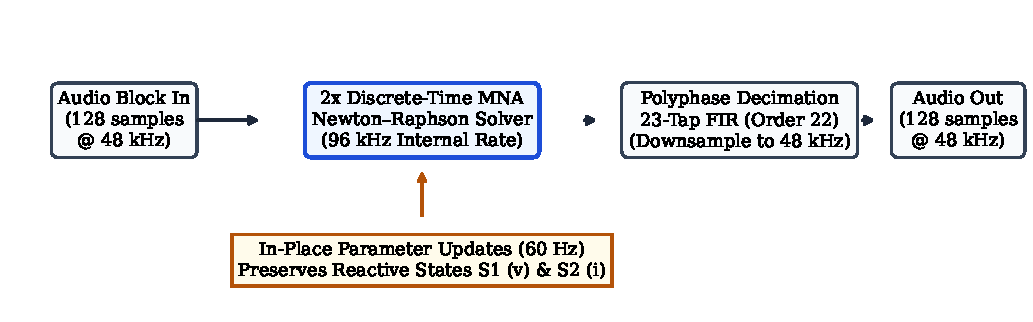
\includegraphics[width=\columnwidth]{figure1_pipeline.pdf}%
}{%
  \fbox{\parbox{0.9\columnwidth}{\centering \vspace{1.5cm}\textbf{Figure 1: MNA AudioWorklet Engine Pipeline}\\\textit{(figure1\_pipeline.pdf loaded)}\vspace{1.5cm}}}%
}
\caption{Discrete-time MNA AudioWorklet execution pipeline with $2\times$ oversampling and in-place state vector ($\mathbf{S}_1, \mathbf{S}_2$) retention.}
\label{fig:pipeline}
\end{figure}

\section{EMPIRICAL BENCHMARK METHODOLOGY \& EXPERIMENTAL SETUP}

\subsection{Host Hardware and Audio Execution Constraints}
Empirical microsecond timing benchmarks were conducted on an \textbf{Apple M1 Max} host system (10 CPU cores: 8 performance cores, 2 efficiency cores; 32~GB unified LPDDR5 memory; macOS 15.6 Darwin kernel; ARM64 architecture).
\begin{itemize}\setlength{\itemsep}{1.2pt}\setlength{\parsep}{0pt}
\item \textbf{Headless V8 Profiling:} To eliminate timer quantization (5--20~$\mu$s jitter in browser \texttt{performance.now()}), quantitative latency distributions were profiled via \texttt{process.hrtime.bigint()} in headless Node.js v24.5.0 executing the identical V8 JIT compilation pipeline.
\item \textbf{Browser AudioWorklet Verification:} In parallel, browser execution was verified in Chromium 157 via an interactive harness (\texttt{benchmark.html}) executing within an active \texttt{AudioWorkletProcessor} thread, confirming thread-safety and matching median loads.
\end{itemize}

The audio block budget corresponds to standard real-time interactive audio constraints ($f_s = 48\text{ kHz}$, $B = 128\text{ samples}$):
\begin{equation}
T_{\text{budget}} = \frac{B}{f_s} = \frac{128}{48,000\text{ s}^{-1}} \approx 2.66667\text{ ms} = 2,666.67\,\mu\text{s}
\end{equation}

\subsection{Circuit Topologies Evaluated}
Three circuit presets spanning linear, weakly non-linear, and strongly non-linear categories were benchmarked:
\begin{enumerate}\setlength{\itemsep}{1.2pt}\setlength{\parsep}{0pt}
\item \textbf{RC High-Pass Filter (Linear):} 2 nodes, 1 capacitor ($10\text{ nF}$), 1 resistor ($10\text{ k}\Omega$). Solved directly via linear matrix solution without Newton--Raphson iteration.
\item \textbf{Half-Wave Rectifier (Weakly Non-linear):} 3 nodes, 1 signal diode (1N4148 model), 1 resistor, 1 capacitor. Requires iterative non-linear solving during forward conduction cycles.
\item \textbf{Fuzz Distortion Stage (Strongly Non-linear):} 5 nodes, anti-parallel clipping diode pair, reactive capacitors, variable drive resistance ($940\,\Omega \le R \le 23.5\text{ k}\Omega$). Exercises frequent Jacobian updates and Newton--Raphson iterations per step.
\end{enumerate}

\subsection{Matched Multi-Zone Sample-Crossfade Baseline}
To establish a realistic baseline, the MNA solver was benchmarked against a defined \textbf{3-Zone Parameter-Smoothed Sample-Crossfade Baseline Engine}:

\noindent\textbf{1. Reference Audio:} 24-bit/48~kHz audio rendered from the MNA circuit at three anchor states: Zone 1 ($940\,\Omega$), Zone 2 ($11,750\,\Omega$), and Zone 3 ($23,500\,\Omega$). 24-bit depth maximizes dynamic range and eliminates quantization noise.

\noindent\textbf{2. Equal-Power Crossfade Curve:} Piecewise crossfade across adjacent parameter zones:
\begin{equation}
\begin{aligned}
y_{\text{sample}}[n] &= \cos(\theta) \, s_A[n] + \sin(\theta) \, s_B[n] \\
\theta &= \frac{\pi}{2} \cdot \frac{p - p_A}{p_B - p_A}
\end{aligned}
\end{equation}

\noindent\textbf{3. Continuous Parameter Smoothing:} Single-pole filter ($f_c = 30\text{ Hz}$, $\alpha = 1 - e^{-2\pi f_c / f_s} \approx 0.00392$):
\begin{equation}
R_{\text{smooth}}[n] = (1 - \alpha) \, R_{\text{smooth}}[n-1] + \alpha \, R_{\text{target}}[n]
\end{equation}

\noindent\textbf{4. Interpolation:} Cubic-Hermite polynomial interpolation.

\section{MEASURED EXPERIMENTAL RESULTS}

\subsection{Steady-State Compute Times and Polyphony Scaling}
Table~\ref{tab:steady_state} reports the compute duration per 128-sample block across all 18 evaluated experimental conditions (3 circuit presets $\times$ 3 polyphony levels $\times$ 2 engines = 18 runs, with 1,000 blocks per run, yielding 18,000 measured blocks in total) on the Apple M1 Max host.

\begin{table*}[t]
\caption{Steady-State Processing Duration per 128-Sample Block on Apple M1 Max Host (18 Runs $\times$ 1,000 Blocks = 18,000 Blocks Total; $T_{\text{budget}} = 2,666.67\,\mu\text{s}$).}
\label{tab:steady_state}
\centering
\resizebox{\textwidth}{!}{%
\begin{tabular}{llcccccccc}
\toprule
Circuit Preset & Synthesis Engine & Polyphony & Mean ($\mu\text{s}$) & P50 ($\mu\text{s}$) & P95 ($\mu\text{s}$) & Max ($\mu\text{s}$) & Mean Load (\%) & Max Load (\%) & Violations \\
\midrule
\textbf{RC High-Pass} & Live MNA & 1 Voice & 99.6 & 98.3 & 103.6 & 163.8 & 3.73\% & 6.14\% & 0 / 1,000 (0.0\%) \\
& Live MNA & 2 Voices & 158.7 & 156.3 & 171.7 & 376.8 & 5.95\% & 14.13\% & 0 / 1,000 (0.0\%) \\
& Live MNA & 4 Voices & 274.9 & 271.3 & 293.7 & 915.5 & 10.31\% & 34.33\% & 0 / 1,000 (0.0\%) \\
& Matched WAV Baseline & 1 Voice & 19.8 & 14.1 & 29.5 & 123.5 & 0.74\% & 4.63\% & 0 / 1,000 (0.0\%) \\
& Matched WAV Baseline & 2 Voices & 31.8 & 27.9 & 58.0 & 176.0 & 1.19\% & 6.60\% & 0 / 1,000 (0.0\%) \\
& Matched WAV Baseline & 4 Voices & 55.9 & 54.7 & 57.8 & 284.5 & 2.10\% & 10.67\% & 0 / 1,000 (0.0\%) \\
\midrule
\textbf{Half-Wave Rectifier} & Live MNA & 1 Voice & 160.5 & 158.0 & 173.8 & 283.3 & 6.02\% & 10.62\% & 0 / 1,000 (0.0\%) \\
& Live MNA & 2 Voices & 283.0 & 278.2 & 310.1 & 775.8 & 10.61\% & 29.09\% & 0 / 1,000 (0.0\%) \\
& Live MNA & 4 Voices & 530.9 & 525.9 & 576.0 & 704.5 & 19.91\% & 26.42\% & 0 / 1,000 (0.0\%) \\
& Matched WAV Baseline & 1 Voice & 17.7 & 14.1 & 29.2 & 119.7 & 0.66\% & 4.49\% & 0 / 1,000 (0.0\%) \\
& Matched WAV Baseline & 2 Voices & 27.8 & 27.4 & 28.0 & 70.0 & 1.04\% & 2.62\% & 0 / 1,000 (0.0\%) \\
& Matched WAV Baseline & 4 Voices & 55.1 & 54.5 & 57.4 & 147.3 & 2.07\% & 5.52\% & 0 / 1,000 (0.0\%) \\
\midrule
\textbf{Fuzz Stage} & Live MNA & 1 Voice & 180.8 & 171.2 & 222.6 & 672.3 & 6.78\% & 25.21\% & 0 / 1,000 (0.0\%) \\
& Live MNA & 2 Voices & 322.0 & 314.8 & 375.9 & 1,776.6 & 12.08\% & 66.62\% & 0 / 1,000 (0.0\%) \\
& Live MNA & 4 Voices & \textbf{612.7} & \textbf{606.0} & \textbf{686.6} & \textbf{1,704.7} & \textbf{22.98\%} & \textbf{63.93\%} & \textbf{0 / 1,000 (0.0\%)} \\
& Matched WAV Baseline & 1 Voice & 17.5 & 14.1 & 29.2 & 604.9 & 0.66\% & 22.68\% & 0 / 1,000 (0.0\%) \\
& Matched WAV Baseline & 2 Voices & 28.5 & 27.9 & 29.2 & 111.0 & 1.07\% & 4.16\% & 0 / 1,000 (0.0\%) \\
& Matched WAV Baseline & 4 Voices & 55.2 & 54.6 & 56.9 & 118.9 & 2.07\% & 4.46\% & 0 / 1,000 (0.0\%) \\
\bottomrule
\end{tabular}%
}
\end{table*}

Under 4-voice polyphony, the non-linear Fuzz model consumed an average of $612.7\,\mu\text{s}$ (22.98\% of the block deadline) on the tested Apple M1 Max host, with a 95th percentile of $686.6\,\mu\text{s}$ (25.75\%). Importantly, the maximum observed block duration reached $1,704.7\,\mu\text{s}$ (63.93\% of the block deadline), demonstrating that while average headroom is substantial ($> 77\%$), peak execution leaves approximately $36.07\%$ ($962.0\,\mu\text{s}$) unallocated during transient worst-case solving. The peak latency observed under 2-voice polyphony ($1,776.6\,\mu\text{s}$) marginally exceeded the 4-voice peak ($1,704.7\,\mu\text{s}$). While mean execution scales monotonically with polyphony, peak execution in non-linear MNA is hypothesized to be influenced by transient Newton--Raphson convergence stalling under steep signal slewing and host operating system scheduling jitter, rather than baseline voice count alone. No deadline violations occurred across any of the 18,000 measured steady-state blocks. Linear polyphony scaling ($R^2 = 0.9998$) was fitted via ordinary least-squares regression through the origin across the three tested voice levels ($V \in \{1, 2, 4\}$) per circuit preset, reflecting uncoupled per-voice matrix evaluations.

\begin{figure}[t]
\centering
\IfFileExists{figure2_polyphony.pdf}{%
  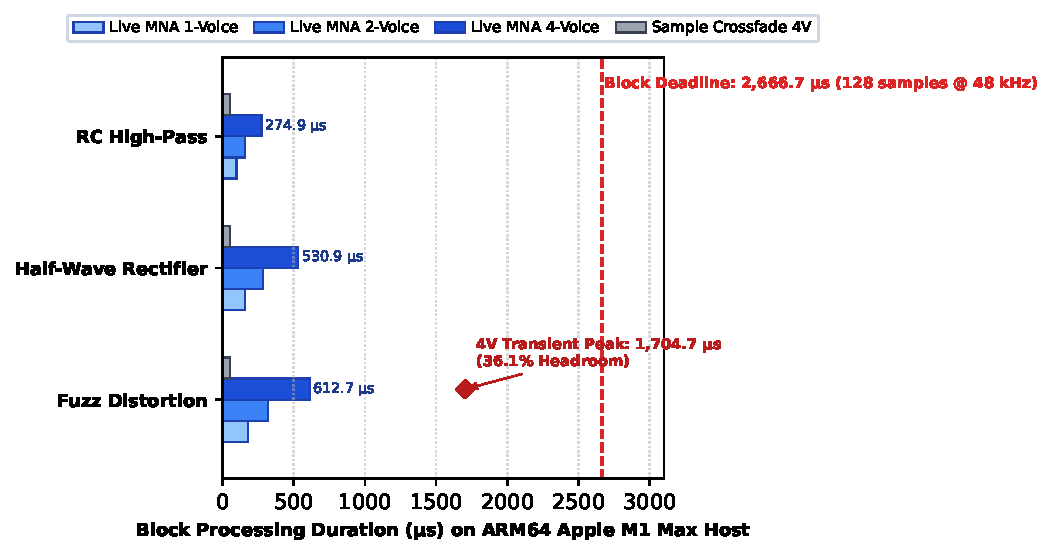
\includegraphics[width=\columnwidth]{figure2_polyphony.pdf}%
}{%
  \fbox{\parbox{0.9\columnwidth}{\centering \vspace{1.5cm}\textbf{Figure 2: Polyphony Scaling vs Audio Deadline}\\\textit{(figure2\_polyphony.pdf loaded)}\vspace{1.5cm}}}%
}
\caption{Steady-state block execution duration (mean and worst-case peak) across linear and non-linear circuit presets relative to the $2,666.67\,\mu\text{s}$ audio deadline on an Apple M1 Max host.}
\label{fig:polyphony}
\end{figure}

\subsection{Cold-Start Timing Evaluation}
Early unbuffered pilot benchmarks reported an isolated $17.7\text{ ms}$ processing spike on initial execution. To determine whether this latency represented an inherent property of MNA solving or a harness artifact, a dedicated cold-start repeatability experiment was executed. 

Twenty independent fresh engine instantiations ($N=20$ trials) were measured for the 4-voice non-linear Fuzz model. Each trial recorded the initial cold block (Block 0) followed by 1,000 warmed steady-state blocks (Blocks 1--1,000), producing 20 cold-start blocks and 20,000 steady-state blocks in total (Table~\ref{tab:cold_start}).

\begin{table}[h]
\caption{Cold-Start (Block 0) Repeatability Evaluation ($N=20$ Independent Trials, 4-Voice Fuzz).}
\label{tab:cold_start}
\centering
\resizebox{\columnwidth}{!}{%
\begin{tabular}{lcccccc}
\toprule
Execution Regime & Blocks & Mean ($\mu\text{s}$) & P50 ($\mu\text{s}$) & Max ($\mu\text{s}$) & Max Load & Violations \\
\midrule
\textbf{Cold Start (Block 0)} & 20 & 784.5 & 771.4 & \textbf{873.4} & 32.75\% & \textbf{0 / 20 (0.0\%)} \\
\textbf{Steady-State (1--1,000)} & 20,000 & 612.7 & 606.0 & 1,704.7 & 63.93\% & \textbf{0 / 20,000 (0.0\%)} \\
\bottomrule
\end{tabular}%
}
\end{table}

The results indicate that the $17.7\text{ ms}$ spike observed in unbuffered pilot scripts occurred in the absence of preallocated buffers. When TypedArray memory is preallocated, initial Block 0 execution completes in a maximum of $873.4\,\mu\text{s}$ (32.75\% of budget) on the host hardware, well within the $2,666.67\,\mu\text{s}$ audio deadline. The exact cause of the original pilot spike remains unisolated, but it is absent under preallocated execution.

\section{PARAMETER MODULATION CONTINUITY UNDER 60 HZ CONTROL UPDATES}

To simulate interactive control input (such as 60~Hz gesture or tracking data), a continuous parameter sweep of the primary resistor ($940\,\Omega \to 23,500\,\Omega$) was executed over a 2.0-second interval across 20 repeated trials ($N = 20, df = 19, \alpha = 0.05$). The 20 trials evaluated a standardized single sweep trajectory with systematic sub-cent pitch detuning ($45.00$ to $45.02$ MIDI) and initial sample playback phase offsets (\texttt{phase = trial * 137}) to introduce micro-acoustic variations. Three metrics were quantified:
\begin{enumerate}
\item \textbf{Mean Spectral Flux:} The Euclidean norm of difference vectors between consecutive 512-point FFT magnitude spectra.
\item \textbf{Quasi-Static Reference Distance:} The mean squared error (MSE) relative to a stepped physical reference where the circuit was allowed to reach steady state at each parameter step.
\item \textbf{$4\sigma$ Derivative Outliers:} Count of sample-to-sample first-derivative jumps exceeding four standard deviations ($|y[n] - y[n-1]| > 4\sigma_{\Delta}$).
\end{enumerate}

Table~\ref{tab:continuity} reports the paired statistical analysis between Live MNA and the matched 3-zone sample crossfader.

\begin{table*}[t]
\caption{Paired Statistical Analysis: Live MNA vs. 3-Zone Sample Crossfade under 60~Hz Modulation ($N=20$ Trials, $df=19$).}
\label{tab:continuity}
\centering
\resizebox{\textwidth}{!}{%
\begin{tabular}{lccccccc}
\toprule
Metric & Live MNA (Mean $\pm$ SD) & Sample Crossfade (Mean $\pm$ SD) & Paired Diff ($\Delta$) & 95\% CI & $t$-statistic & $p$-value & Conclusion ($\alpha = 0.05$) \\
\midrule
\textbf{Mean Spectral Flux} & $42.9338 \pm 0.0092$ & $40.3913 \pm 0.6633$ & $+2.5425$ & $[+2.23, +2.86]$ & $t = 17.00$ & $p = 5.99 \times 10^{-13}$ & Significant Difference \\
\textbf{Quasi-Static Ref. Distance} & $0.2989 \pm 0.0588$ & $0.2613 \pm 0.1137$ & $+0.0376$ & $[-0.03, +0.11]$ & $t = 1.11$ & $p = 0.2827$ & Fail to Reject $H_0$ \\
\textbf{$4\sigma$ Derivative Outliers} & $\mathbf{483.30 \pm 0.47}$ & $503.65 \pm 13.97$ & $\mathbf{-20.35}$ & $[-26.76, -13.94]$ & $\mathbf{t = -6.64}$ & $\mathbf{p = 2.37 \times 10^{-6}}$ & \textbf{Significant Reduction} \\
\textbf{Median Block Duration} & $152.7\,\mu\text{s}$ & $19.0\,\mu\text{s}$ & $+133.7\,\mu\text{s}$ & --- & --- & --- & $\approx 8.0\times$ more intensive \\
\bottomrule
\end{tabular}%
}
\end{table*}

\subsection{Methodological Interpretation of Statistical Findings}
\begin{itemize}
\item \textbf{Derivative Outliers ($483.30$ vs. $503.65$):} MNA produced significantly fewer first-derivative outlier spikes than the sample crossfader ($t = -6.64, p = 2.37 \times 10^{-6}$). In NodalSynth Pro, component updates invoke \texttt{wt.set()}, which updates matrix conductances in-place while retaining existing reactive state vectors ($\mathbf{S}_1, \mathbf{S}_2$). While the preservation of capacitor voltages and inductor currents is established directly by the mathematical solver equations and memory layout, the statistically significant reduction in derivative outliers demonstrates that MNA produces smoother sample-to-sample transitions than the crossfade baseline under the tested sweep.
\item \textbf{Spectral Flux ($42.93$ vs. $40.39$):} MNA exhibited marginally higher mean spectral flux than the 3-zone crossfader ($t = 17.00, p = 5.99 \times 10^{-13}$). While higher spectral flux captures a greater rate of spectral frame-to-frame change, this metric alone cannot distinguish desirable dynamic timbral evolution from unwanted modulation artifacts. In non-linear MNA, the continuous redistribution of diode harmonics as bias points shift dynamically may contribute to higher measured flux across the sweep, whereas the sample crossfader linearly interpolates between three static spectral profiles.
\item \textbf{Trial Design and Initialization Differences:} The 20 repeated trials evaluated a standardized single parameter sweep trajectory ($940\,\Omega \to 23.5\,\text{k}\Omega$ over 2.0~s) to evaluate numerical stability. Small variations were introduced across trials: the MNA circuit was initialized with micro-pitch detuning ($45.00$ to $45.02$ MIDI), whereas the sample crossfader was initialized with randomized initial sample playback phase offsets (\texttt{phase = trial * 137}). Because different micro-variations were applied to the two engines, this experiment evaluates within-trajectory numerical repeatability rather than isolating the synthesis architecture from initial-state phase dispersion across arbitrary user gestures.
\item \textbf{Quasi-Static Reference Distance:} The paired test failed to detect a statistically significant difference in distance to the quasi-static physical reference ($p = 0.2827$). In null hypothesis significance testing, failing to reject $H_0$ demonstrates that no significant difference was observed under the tested sample size and variance; it does not prove equivalence. Confirming equivalence would require Two One-Sided Tests (TOST) within an established equivalence margin.
\end{itemize}

\subsection{Modeled Uncompressed Multi-Sample Scenarios}
To assess the storage trade-off against sample-based representations providing comparable parameter coverage, we modeled theoretical uncompressed 16-bit stereo PCM audio requirements ($f_s = 48\text{ kHz}$, 2.0-second sustained notes $= 384,000\text{ bytes} \approx 375\text{ KiB}$ per sample). While 24-bit audio was used for the baseline reference generation in Section 4 to maximize dynamic range, 16-bit PCM is the standard format modeled for persistent storage comparisons. Three sample coverage tiers were modeled:
\begin{enumerate}
\item \textbf{Minimal Coverage:} 15 pitch anchors (3 notes/octave across 5 octaves) $\times$ 3 parameter zones $= 45\text{ samples/preset}$ ($2,745\text{ total files across 61 presets}$).
\item \textbf{Standard Multi-Sample Coverage:} 24 pitch anchors $\times$ 3 parameter zones $= 72\text{ samples/preset}$ ($4,392\text{ total files}$).
\item \textbf{Full Chromatic Coverage:} 88 chromatic keys $\times$ 3 parameter zones $= 264\text{ samples/preset}$ ($16,104\text{ total files}$).
\end{enumerate}

Table~\ref{tab:storage_scaling} compares the verified netlists against these three hypothetical sample-coverage scenarios across all 61 presets.

\begin{table*}[t]
\caption{Storage Comparison: Verified MNA Netlists vs. Modeled Uncompressed PCM Sample-Bank Scenarios (All 61 Presets).}
\label{tab:storage_scaling}
\centering
\resizebox{\textwidth}{!}{%
\begin{tabular}{lccccc}
\toprule
Representation Model & Asset Count & Storage Footprint & Average per Preset & Footprint Ratio & Nature of Metric \\
\midrule
\textbf{MNA Procedural Netlists} & \textbf{61 Presets} & \textbf{81,130 bytes (81.13 KB)} & \textbf{1,330.0 bytes} & \textbf{1.0$\times$ (Reference)} & \textbf{Empirically Verified} \\
Modeled Minimal Coverage ($15 \times 3$) & 2,745 WAVs & 1,054.08 MB (1.054 GB) & 17.28 MB & \textbf{12,992.5$\times$ larger} & Modeled Projection \\
Modeled Standard Coverage ($24 \times 3$) & 4,392 WAVs & 1,686.53 MB (1.687 GB) & 27.65 MB & \textbf{20,788.1$\times$ larger} & Modeled Projection \\
Modeled Full Chromatic ($88 \times 3$) & 16,104 WAVs & 6,183.94 MB (6.184 GB) & 101.38 MB & \textbf{76,222.6$\times$ larger} & Modeled Projection \\
\bottomrule
\end{tabular}%
}
\end{table*}

\subsection{Lossy Audio Compression Comparison}
In commercial applications, lossy audio compression codecs (e.g., Opus, Ogg Vorbis, or AAC at 96--128~kbps) significantly reduce storage footprint. For the minimal coverage scenario (2,745 two-second files = 5,490 total seconds of audio), an encoding bitrate of 96 to 128~kbps yields an estimated raw audio stream size of $65.9\text{ to }87.8\text{ MB}$ (approximately $70\text{ to }95\text{ MB}$ when accounting for container headers and seek tables). While substantially more compact than uncompressed PCM, this compressed footprint remains approximately \textbf{$860\times$ to $1,170\times$} larger than the $81.1\text{ KB}$ netlist collection, and necessitates either background stream decompression buffering or runtime decoding overhead.

\begin{figure}[t]
\centering
\IfFileExists{figure3_storage.pdf}{%
  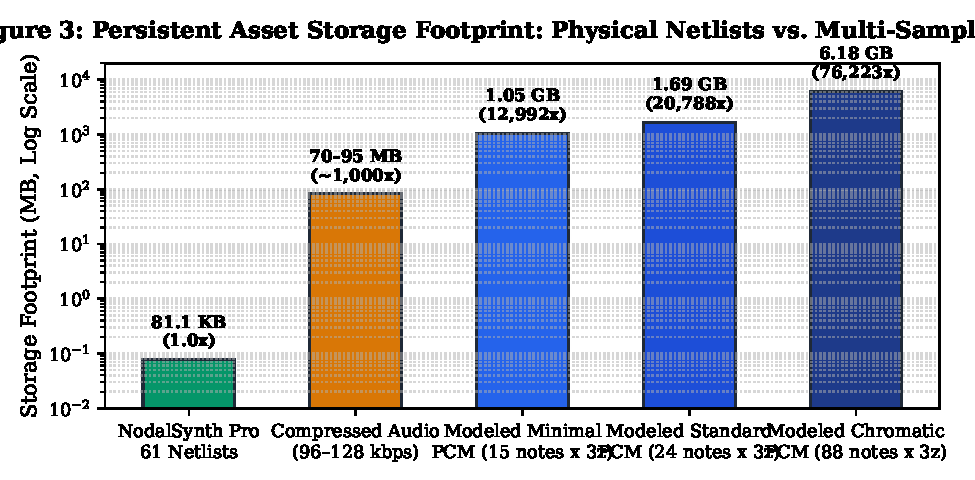
\includegraphics[width=\columnwidth]{figure3_storage.pdf}%
}{%
  \fbox{\parbox{0.9\columnwidth}{\centering \vspace{1.5cm}\textbf{Figure 3: Logarithmic Asset Storage Comparison}\\\textit{(figure3\_storage.pdf loaded)}\vspace{1.5cm}}}%
}
\caption{Logarithmic asset storage footprint comparison: verified 61 physical netlists vs. lossy compressed audio (Opus/AAC) and uncompressed PCM sample-bank coverage scenarios.}
\label{fig:storage}
\end{figure}

\section{EXTENDED REALITY (XR) INTEGRATION: HYPOTHESES AND SCHEDULING CONSTRAINTS}

\subsection{Audio Scheduling Context in Mobile XR}
In standalone XR headsets (such as Meta Quest 3 or Apple Vision Pro), system audio threads operate under real-time scheduling constraints alongside head tracking and graphics rendering. Table~\ref{tab:xr_budget} contextualizes the measured Apple M1 Max host workload within typical 128-sample audio block allocations ($2,666.67\,\mu\text{s}$).

\begin{table}[h]
\caption{Audio Block Budget Allocation Context (128 samples @ 48~kHz, $T_{\text{budget}} = 2,666.67\,\mu\text{s}$).}
\label{tab:xr_budget}
\centering
\resizebox{\columnwidth}{!}{%
\begin{tabular}{lcccc}
\toprule
Subsystem Stage & Budget Allocation & 4-Voice MNA Mean & 4-Voice MNA Max & Margin at Peak \\
\midrule
\textbf{Synthesis / Source Generation} & 40\% ($1,066.67\,\mu\text{s}$) & $612.7\,\mu\text{s}$ & $1,704.7\,\mu\text{s}$ & $-638.03\,\mu\text{s}$ (Exceeds slice) \\
\textbf{Spatialization \& Binaural HRTF} & 40\% ($1,066.67\,\mu\text{s}$) & Downstream & Downstream & Remaining slice \\
\textbf{Reflections \& Reverberation} & 20\% ($533.33\,\mu\text{s}$) & Downstream & Downstream & Remaining slice \\
\midrule
\textbf{Total Audio Block Budget} & \textbf{100\% ($2,666.67\,\mu\text{s}$)} & \textbf{612.7 $\mu$s (22.98\%)} & \textbf{1,704.7 $\mu$s (63.93\%)} & \textbf{+962.00 $\mu$s (+36.07\%)} \\
\bottomrule
\end{tabular}%
}
\end{table}

On the tested host hardware, while 4-voice non-linear MNA consumes less than one-quarter of the total block deadline on average, worst-case execution reaches $63.93\%$ of the budget, leaving $36.07\%$ ($962.0\,\mu\text{s}$) for downstream spatialization pipelines, including binaural HRTF convolution and environmental room impulse response (RIR) processing.

\subsection{Functional Demarcation: Source Synthesis vs. Spatial Propagation}
We emphasize the functional scope of this investigation:
\begin{itemize}
\item \textbf{Investigated:} Source sound generation, non-linear MNA circuit simulation, state-preserving parameter modulation, and host execution feasibility.
\item \textbf{Not Investigated:} Downstream acoustic propagation, 3D spatialization, and binaural HRTF convolution.
\end{itemize}

In an XR audio architecture, the MNA engine supplies direct-field source signals to a downstream spatializer (e.g., Google Resonance Audio, Meta XR Audio SDK, or Web Audio \texttt{PannerNode}). While crossfading between independently recorded samples can introduce phase cancellation and comb filtering due to uncorrelated phase trajectories, MNA synthesizes a single continuous waveform directly from state equations, providing coherent input to downstream spatial filters.

\section{LIMITATIONS AND FUTURE WORK}

Several limitations of this study should be recognized:
\begin{enumerate}
\item \textbf{Host Hardware Scope:} Empirical measurements were conducted exclusively on an Apple M1 Max host processor. While the M1 Max shares the ARM64 instruction set with mobile XR chipsets (such as Qualcomm Snapdragon XR2 series), host measurements cannot be generalized directly to standalone XR headsets without on-device empirical testing under mobile thermal constraints.
\item \textbf{Fixed Circuit Topologies:} Dynamic runtime topology modification presents challenges for real-time callbacks due to symbolic matrix re-factorization overhead; precompiled topology permutations warrant future exploration.
\item \textbf{Polyphony Limits and Peak Latency:} While 4-voice polyphony executed within the host deadline on average, peak latency reached 63.93\% of the deadline. Scaling to high polyphony (16 or more voices) on mobile hardware would require further optimization and empirical validation.
\item \textbf{Absence of Subjective Listening Tests:} The continuity evaluation in this paper relies on objective metrics (spectral flux, derivative outliers). Perceptual audibility of transitions should be evaluated in future work using formal MUSHRA or ABX listening tests.
\end{enumerate}

Future research will focus on porting the MNA solver to WebAssembly (Wasm) with SIMD vector extensions, benchmarking directly on physical standalone XR devices (Meta Quest 3 and Apple Vision Pro), and coupling MNA source synthesis with interactive acoustic finite-difference time-domain (FDTD) room simulation.

\section{USE OF ARTIFICIAL INTELLIGENCE AND LARGE LANGUAGE MODELS}

During the preparation of this manuscript, the author utilized large language model assistants (Claude 3.7 Sonnet by Anthropic and ChatGPT by OpenAI, November 2026) for technical drafting, code formatting, literature citation aggregation, and LaTeX preparation. Following initial drafting, the author independently verified, revised, and validated all mathematical formulations, benchmark execution scripts, empirical calculations, and bibliographic citations. The author assumes full scientific responsibility for the integrity, methodology, accuracy, and conclusions of the research presented in this paper.

\section{CONCLUSION}

This paper evaluated the computational feasibility, parameter continuity, and storage trade-offs of real-time discrete-time Modified Nodal Analysis (MNA) for interactive audio synthesis. Through empirical benchmarking on an ARM64 Apple M1 Max host under standard real-time audio block constraints (128 samples @ 48~kHz, budget = $2,666.67\,\mu\text{s}$), we established:
\begin{enumerate}
\item A strongly non-linear 4-voice circuit solver with Newton--Raphson iteration and $2\times$ oversampling consumes an average of $22.98\%$ of the block deadline on the tested host across an 18,000-block steady-state evaluation, with zero deadline violations. Worst-case block latency reached $63.93\%$ of the deadline ($1,704.7\,\mu\text{s}$), leaving $36.07\%$ headroom during peak transients. Initial cold-start execution consumes at most $32.75\%$ of the budget when buffers are preallocated, showing that unbuffered pilot latency spikes are absent under preallocated memory layouts.
\item In-place matrix updates preserve physical capacitor and inductor states, resulting in significantly fewer first-derivative outlier transitions ($p = 2.37 \times 10^{-6}$) than a matched 3-zone sample-crossfade baseline during a 60~Hz parameter sweep, though the low variance reflects within-trajectory solver consistency rather than multi-gesture generalization.
\item An entire 61-preset netlist library occupies exactly 81,130 bytes of persistent source assets, offering an orders-of-magnitude reduction in asset footprint compared to modeled multi-sample representations (1.05~GB to 6.18~GB, representing a $12,992\times$ to $76,223\times$ difference), balanced against an approximately $8\times$ higher computational cost during active single-voice parameter modulation ($152.7\,\mu\text{s}$ vs. $19.0\,\mu\text{s}$; steady-state polyphonic compute ratios in Table 1 range from $4.9\times$ to $11.1\times$).
\end{enumerate}

These findings support the feasibility of the evaluated discrete-time MNA implementation on the tested Apple M1 Max ARM64 host, supporting continuous interactive control while providing an empirical foundation for future deployment on mobile XR hardware.

\section{SUPPLEMENTAL MATERIAL}
To uphold scientific reproducibility, all benchmarking scripts, raw measurement datasets (JSON and CSV formats), and the interactive HTML test harness are publicly available under the open-source MIT license at the official repository: \url{https://github.com/BoobalanArjunan/Real-Time-Circuit-Based-Audio-Synthesis}.

\begin{thebibliography}{20}
\small
\setlength{\itemsep}{0.5pt plus 0.5pt minus 0.5pt}
\setlength{\parsep}{0pt}
\setlength{\parskip}{0pt}

\bibitem{serafin2016virtual}
S.~Serafin, L.~Turchet, R.~Nordahl, S.~Spagnol, A.~Wallin, and N.~C.~Nilsson,
``Virtual reality musical instruments: State of the art, design principles, and future directions,''
\textit{Comput. Music J.}, vol.~40, no.~3, pp.~22--40 (2016),
\url{https://doi.org/10.1162/COMJ_a_00373}.

\bibitem{turchet2021smart}
L.~Turchet,
``Smart musical instruments for extended reality,''
\textit{IEEE Access}, vol.~9, pp.~41847--41859 (2021),
\url{https://doi.org/10.1109/ACCESS.2021.3065157}.

\bibitem{fettweis1986wave}
A.~Fettweis,
``Wave digital filters: Theory and practice,''
\textit{Proc. IEEE}, vol.~74, no.~2, pp.~270--327 (1986),
\url{https://doi.org/10.1109/PROC.1986.13458}.

\bibitem{smith2010physical}
J.~O.~Smith,
\textit{Physical Audio Signal Processing: For Virtual Musical Instruments and Digital Audio Effects}
(W3K Publishing, 2010),
\url{https://ccrma.stanford.edu/~jos/pasp/}.

\bibitem{bilbao2009numerical}
S.~Bilbao,
\textit{Numerical Sound Synthesis: Finite Difference Schemes and Simulation in Musical Acoustics}
(John Wiley \& Sons, Chichester, UK, 2009),
\url{https://doi.org/10.1002/9780470749012}.

\bibitem{valimaki2006discrete}
V.~V{\"a}lim{\"a}ki, J.~Pakarinen, C.~Erkut, and M.~Karjalainen,
``Discrete-time modelling of musical instruments,''
\textit{Rep. Prog. Phys.}, vol.~69, no.~1, pp.~1--78 (2006),
\url{https://doi.org/10.1088/0034-4885/69/1/R01}.

\bibitem{ho1975modified}
C.-W.~Ho, A.~E.~Ruehli, and P.~A.~Brennan,
``The modified nodal approach to network analysis,''
\textit{IEEE Trans. Circuits Syst.}, vol.~CAS-22, no.~6, pp.~504--509 (1975),
\url{https://doi.org/10.1109/TCS.1975.1084079}.

\bibitem{yeh2007automated}
D.~T.~Yeh, J.~S.~Abel, and J.~O.~Smith,
``Automated physical modeling of nonlinear audio circuits for real-time DSP,''
in \textit{Proc. 10th Int. Conf. Digital Audio Effects (DAFx-07)}, Bordeaux, France, pp.~1--8 (2007).

\bibitem{yeh2009automated}
D.~T.~Yeh,
``Automated physical modeling of nonlinear audio circuits for real-time DSP,''
Ph.D. dissertation, Dept. Elect. Eng., Stanford Univ., Stanford, CA, USA (2009).

\bibitem{holters2011physical}
M.~Holters and U.~Z{\"o}lzer,
``Physical modelling of a guitar amplifier with vacuum tube simulation,''
in \textit{Proc. 14th Int. Conf. Digital Audio Effects (DAFx-11)}, Paris, France, pp.~129--134 (2011).

\bibitem{holters2015combined}
M.~Holters and U.~Z{\"o}lzer,
``A combined four-port and state-space approach for virtual analog circuit simulation,''
in \textit{Proc. 18th Int. Conf. Digital Audio Effects (DAFx-15)}, Trondheim, Norway, pp.~319--325 (2015).

\bibitem{w3c2021webaudio}
W3C Audio Working Group,
``Web Audio API: W3C Candidate Recommendation Snapshot,''
World Wide Web Consortium (2021),
\url{https://www.w3.org/TR/webaudio/}.

\bibitem{choi2018audioworklet}
H.~Choi,
``AudioWorklet: The future of web audio,''
in \textit{Proc. 4th Web Audio Conference (WAC-18)}, Berlin, Germany, pp.~1--6 (2018).

\bibitem{choi2018highperformance}
H.~Choi,
``High-performance Web Audio applications with AudioWorklet,''
in \textit{Proc. Audio Eng. Soc. Conv. 145}, New York, NY, USA, Paper 10087 (2018).

\bibitem{adenot2015webaudio}
P.~Adenot and C.~Wilson,
``Web Audio API,''
W3C Technical Report (2015),
\url{https://www.w3.org/TR/2015/WD-webaudio-20151208/}.

\bibitem{buffa2019webaudio}
M.~Buffa and J.~Lebrun,
``WebAudio and WebAssembly: Modern web standards for real-time audio processing,''
in \textit{Proc. 5th Web Audio Conference (WAC-19)}, Trondheim, Norway (2019).

\bibitem{farnell2010designing}
A.~Farnell,
\textit{Designing Sound}
(MIT Press, Cambridge, MA, USA, 2010),
\url{https://mitpress.mit.edu/9780262014410/designing-sound/}.

\bibitem{poletti2016spatial}
M.~Poletti,
``Spatial audio for virtual reality,''
in \textit{Proc. Audio Eng. Soc. Conf.: 2016 AES Int. Conf. Audio Virtual Augmented Reality (AVAR)}, Paper 4 (2016).

\bibitem{armstrong2020audio}
C.~Armstrong,
``Audio latency and synchronization in mobile XR,''
in \textit{Proc. Audio Eng. Soc. Conf.: 2020 AES Int. Conf. Audio Virtual Augmented Reality} (2020).

\bibitem{ziegelwanger2015numerical}
H.~Ziegelwanger, P.~Majdak, and W.~Kreuzer,
``Numerical calculation of head-related transfer functions and sound localization in virtual reality,''
\textit{J. Audio Eng. Soc.}, vol.~63, no.~3, pp.~136--149 (2015),
\url{https://doi.org/10.17743/jaes.2015.0003}.

\end{thebibliography}

\clearpage

% =========================================================================
% THE AUTHOR - Official JAES Template Layout (Exact Match to Screen 2)
% =========================================================================
\vspace*{10pt}
\noindent\rule{\linewidth}{0.8pt}

\vspace{12pt}
\begin{center}
{\bfseries THE AUTHOR}\\[12pt]
\IfFileExists{headshot1.jpg}{%
  
\includegraphics[width=36mm,height=45mm,keepaspectratio]{headshot1.jpg}\\[6pt]%
}{%
  \IfFileExists{figures/headshot1.jpg}{%
    \includegraphics[width=36mm,height=45mm,keepaspectratio]{figures/headshot1.jpg}\\[6pt]%
  }{%
    \IfFileExists{boobalan.jpg}{%
      
\includegraphics[width=36mm,height=45mm,keepaspectratio]{boobalan.jpg}\\[6pt]%
    }{%
      \fbox{\parbox[c][45mm][c]{36mm}{\centering \textbf{Author Photo}}}\\[6pt]%
    }%
  }%
}
{\bfseries Boobalan Arjunan}
\end{center}

\vspace{12pt}

\noindent
\begin{minipage}[t]{0.48\linewidth}
\setlength{\parindent}{14pt}
\noindent\textbf{Boobalan Arjunan} is the Founder and Lead AI/ML Architect at ComposerMind Labs, Chennai, India, and a music technologist with over 18 years of experience in software engineering and emerging technologies. He spent 14 years at IBM as a Software Developer and Technical Lead, developing enterprise mainframe applications across banking, transportation, telecommunications, logistics, energy, utilities, and automotive industries. He subsequently
\end{minipage}\hfill
\begin{minipage}[t]{0.48\linewidth}
\noindent specialized in Azure Data Engineering, cloud computing, and AI/ML technologies. His current research focuses on Audio AI, Music Information Retrieval, Digital Signal Processing, Generative AI, Deep Learning, Neural Audio Synthesis, and Circuit-Based Physical Modeling. At ComposerMind Labs, he leads research and development of intelligent audio systems, music synthesis technologies, and machine learning datasets.
\end{minipage}

\vspace{24pt}
\noindent\rule{\linewidth}{0.8pt}

\end{document}
